% ============================================================
%  FA-KGD -- Milestone 2 Slides (Technical Approach)
%  CS 231N, Stanford, Spring 2026
% ============================================================
\documentclass[aspectratio=169]{beamer}

\usetheme{metropolis}
\usepackage{amsmath,amssymb,amsfonts}
\usepackage{booktabs}
\usepackage{graphicx}
\usepackage{xcolor}
\usepackage{hyperref}
\usepackage{tikz}
\usetikzlibrary{arrows.meta,positioning,calc}

\graphicspath{{figures/}}

\definecolor{stanfordred}{RGB}{140,21,21}
\definecolor{deepnavy}{RGB}{26,44,71}
\definecolor{softblue}{RGB}{70,130,180}
\definecolor{softgray}{RGB}{245,247,250}
\setbeamercolor{progress bar}{fg=stanfordred}
\setbeamercolor{title separator}{fg=stanfordred}
\setbeamercolor{alerted text}{fg=stanfordred}
\setbeamerfont{title}{size=\Large}
\setbeamerfont{subtitle}{size=\normalsize}
\setbeamerfont{author}{size=\small}
\setbeamerfont{institute}{size=\small}
\setbeamerfont{date}{size=\small}

\newcommand{\PIGDM}{$\Pi$GDM}
\newcommand{\FAKGD}{FA-KGD}
\newcommand{\hatR}{\hat{\mathbf{R}}}
\newcommand{\hatsig}{\hat{\sigma}}
\newcommand{\muth}{\mu_\theta}

\title{FA-KGD: Frequency-Aware Kalman-Guided Diffusion\\for Accelerated MRI}
\subtitle{Milestone 2 --- Technical Approach}
\author{Carlo Schreiber, Emma Sampietro, Nino Alex Triandafilidis}
\institute{CS 231N --- Stanford University}
\date{May 22, 2026}

\begin{document}

% -----------------------------------------------------------
\begin{frame}[plain]
  \vfill
  {\Large\bfseries FA-KGD: Frequency-Aware Kalman-Guided Diffusion\\for Accelerated MRI\par}
  \vspace{0.5em}
  {\normalsize Milestone 2 --- Technical Approach\par}
  \vspace{0.6em}
  {\color{stanfordred}\rule{0.82\textwidth}{1.2pt}}
  \vspace{0.8em}

  {\small Carlo Schreiber, Emma Sampietro, Nino Alex Triandafilidis\par}
  \vspace{0.35em}
  {\small CS 231N --- Stanford University\par}
  \vspace{0.35em}
  {\small May 22, 2026\par}
  \vfill
\end{frame}

% -----------------------------------------------------------
\begin{frame}{Method overview}
  \begin{center}
    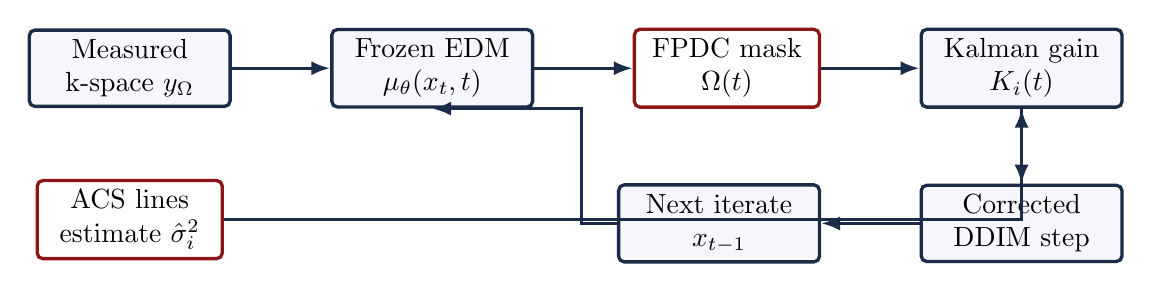
\begin{tikzpicture}[
      node distance=1.0cm,
      box/.style={draw=deepnavy, rounded corners=2pt, fill=softgray, very thick,
                  align=center, minimum width=2.55cm, minimum height=0.85cm},
      smallbox/.style={draw=stanfordred, rounded corners=2pt, fill=white, very thick,
                  align=center, minimum width=2.35cm, minimum height=0.75cm},
      arrow/.style={-{Latex[length=2.4mm]}, very thick, draw=deepnavy}
    ]
      \node[box] (y) {Measured\\k-space $y_\Omega$};
      \node[smallbox, below=0.9cm of y] (acs) {ACS lines\\estimate $\hatsig_i^2$};
      \node[box, right=1.25cm of y] (denoise) {Frozen EDM\\$\muth(x_t,t)$};
      \node[smallbox, right=1.25cm of denoise] (fpdc) {FPDC mask\\$\Omega(t)$};
      \node[box, right=1.25cm of fpdc] (gain) {Kalman gain\\$K_i(t)$};
      \node[box, below=0.95cm of gain] (step) {Corrected\\DDIM step};
      \node[box, left=1.25cm of step] (xnext) {Next iterate\\$x_{t-1}$};

      \draw[arrow] (y) -- (denoise);
      \draw[arrow] (denoise) -- (fpdc);
      \draw[arrow] (fpdc) -- (gain);
      \draw[arrow] (gain) -- (step);
      \draw[arrow] (step) -- (xnext);
      \draw[arrow] (xnext.west) -- ++(-0.45,0) |- (denoise.south);
      \draw[arrow] (acs) -| (gain.south);
    \end{tikzpicture}
  \end{center}
  \vspace{0.4em}
  \textbf{Core idea.} Keep \PIGDM{}'s closed-form posterior-correction scaffold, but make the measurement correction match MRI physics: frequency-dependent noise, coarse-to-fine denoising, and scan-local calibration.
\end{frame}

% -----------------------------------------------------------
\begin{frame}{Design choice 1: frequency-aware Kalman gain}
  \small
  \begin{columns}[T]
    \begin{column}{0.55\textwidth}
      \textbf{Problem with \PIGDM{}.} The baseline assumes a single measurement variance:
      \[
        \mathbf{R}=\sigma_y^2\mathbf{I}.
      \]
      Real multicoil MRI does not behave this way: SNR changes sharply from the ACS center to peripheral k-space, and varies across coils.
      \vspace{0.5em}

      \textbf{FA-KGD correction.} Estimate a diagonal measurement covariance from ACS residuals and use a per-frequency gain:
      \[
        K_i(t)=\frac{\sigma_t^2}{\sigma_t^2+\hatsig_i^2}.
      \]
    \end{column}
    \begin{column}{0.45\textwidth}
      \textbf{Why this should work}
      \begin{itemize}
        \item Early noisy denoising steps trust stable measured frequencies more.
        \item Late steps stop over-fitting high-frequency noisy measurements.
        \item The scan itself supplies the calibration signal; no retraining or extra data.
      \end{itemize}
      \vspace{0.4em}
      \textbf{Implementation target}
      \[
        \begin{aligned}
        \hat{x}^{K}_{t-1}
        &= \muth(x_t) + F_\Omega^H K(t)e_\Omega,\\
        e_\Omega &= y_\Omega-F_\Omega \muth(x_t).
        \end{aligned}
      \]
    \end{column}
  \end{columns}
\end{frame}

% -----------------------------------------------------------
\begin{frame}{Design choice 2: frequency-progressive data consistency}
  \small
  \begin{columns}[T]
    \begin{column}{0.48\textwidth}
      \textbf{Failure mode: DC shock}
      \begin{itemize}
        \item Standard samplers hard-enforce every measured k-space frequency at every denoising step.
        \item Early iterates are coarse; forcing high-frequency residuals to zero injects ringing and can make more steps worse.
      \end{itemize}
      \vspace{0.4em}
      \textbf{Schedule}
      \[
        r(t)=r_{\text{ACS}}+(r_{\max}-r_{\text{ACS}})
        \left(1-\frac{t}{T}\right)^\beta .
      \]
      Only frequencies inside radius $r(t)$ enter the correction.
    \end{column}
    \begin{column}{0.52\textwidth}
      \begin{center}
        
\includegraphics[width=0.94\textwidth]{fig3_scaling_curve.png}
      \end{center}
      \vspace{-0.4em}
      \footnotesize
      Empirical signal to test: \PIGDM{} should plateau or regress as $T$ grows; FA-KGD should turn extra steps into useful correction.
    \end{column}
  \end{columns}
\end{frame}

% -----------------------------------------------------------
\begin{frame}{Design choice 3: conservative online noise refinement}
  \small
  \textbf{Question.} Can we refine $\hatsig_i^2$ during sampling using the residual energy?
  \[
    r_i^{(t)} = y_i - [F_{\Omega(t)}\muth(x_t)]_i
  \]
  \vspace{-0.3em}
  \[
    \hatsig_i^2 \leftarrow \alpha(t)\hatsig_i^2
    +(1-\alpha(t))\max\left(|r_i^{(t)}|^2-\gamma\sigma_t^2,\epsilon\right).
  \]

  \begin{columns}[T]
    \begin{column}{0.5\textwidth}
      \textbf{Design intuition}
      \begin{itemize}
        \item Residual energy mixes true measurement noise with denoiser error.
        \item Subtracting all $\sigma_t^2$ over-corrects when the score network is good.
        \item Default: $\gamma=0$ with EMA smoothing; test $\gamma$ as an ablation.
      \end{itemize}
    \end{column}
    \begin{column}{0.5\textwidth}
      \textbf{Progressive extension}
      \begin{itemize}
        \item Pool ACS statistics across slices in the same 3D volume.
        \item Increases effective samples from $N_c-1$ to $N_z(N_c-1)$.
        \item Keeps training-free inference and adds no neural compute.
      \end{itemize}
    \end{column}
  \end{columns}
\end{frame}

% -----------------------------------------------------------
\begin{frame}{Baselines and ablations}
  \small
  \begin{columns}[T]
    \begin{column}{0.50\textwidth}
      \textbf{Baselines}
      \begin{itemize}
        \item Zero-filled reconstruction: lower bound.
        \item ESPIRiT: classical compressed-sensing MRI.
        \item DPS and ADPS: likelihood-guided diffusion samplers.
        \item \PIGDM{}: primary training-free Kalman-style baseline.
        \item E2E-VarNet: supervised reference, not a fair training-free comparison.
      \end{itemize}
    \end{column}
    \begin{column}{0.50\textwidth}
      \textbf{Ablation logic}
      \begin{center}
      \scriptsize
      \begin{tabular}{@{}l c@{}}
        \toprule
        Variant & Purpose \\
        \midrule
        \PIGDM{} & isotropic covariance baseline \\
        Gain only & isolates ACS noise model \\
        FPDC only & isolates DC schedule \\
        Gain + FPDC & tests interaction/synergy \\
        $\gamma\in\{0,1\}$ & tests bias correction \\
        2D vs 3D ACS & tests volumetric pooling \\
        \bottomrule
      \end{tabular}
      \end{center}
      \vspace{0.2em}
      \footnotesize
      Success requires gains over \PIGDM{} plus component evidence for where they come from.
    \end{column}
  \end{columns}
\end{frame}

% -----------------------------------------------------------
\begin{frame}{Experimental setup}
  \footnotesize
  \begin{columns}[T]
    \begin{column}{0.55\textwidth}
      \textbf{Dataset and model}
      \begin{itemize}
        \item fastMRI multicoil brain and knee.
        \item $R\in\{4,8\}$ masks with ACS center retained.
        \item Frozen pretrained EDM checkpoint; no task-specific training.
        \item Brain is domain-matched; knee tests cross-domain transfer.
      \end{itemize}
      \vspace{0.4em}
      \textbf{Metrics}
      \begin{itemize}
        \item PSNR, SSIM, NMSE against fully sampled ground truth.
        \item Per-band k-space NMSE for frequency-specific behavior.
      \end{itemize}
    \end{column}
    \begin{column}{0.45\textwidth}
      \textbf{Experiment matrix}
      \begin{center}
      \scriptsize
      \begin{tabular}{@{}l c c c@{}}
        \toprule
        Setting & $R$ & Steps & Readout \\
        \midrule
        Brain & 4 & 20, 50, 100 & scaling \\
        Brain & 8 & 50 & harder mask \\
        Knee & 4 & 20 & transfer \\
        Knee & 8 & 20 & stress test \\
        Oracle & 4, 8 & 100 & ablation \\
        \bottomrule
      \end{tabular}
      \end{center}
      \vspace{0.2em}
      \footnotesize
      Report slice mean $\pm$ std and paired deltas vs.\ \PIGDM{}.
    \end{column}
  \end{columns}
\end{frame}

% -----------------------------------------------------------
\begin{frame}{Current evidence to validate the approach}
  \begin{columns}[T]
    \begin{column}{0.49\textwidth}
      
\includegraphics[width=\textwidth]{fig1_reconstruction_comparison.png}
      \vspace{-0.4em}

      \footnotesize
      Qualitative check: FA-KGD reduces residual energy around cortical and ventricular boundaries, where DC shock appears visually.
    \end{column}
    \begin{column}{0.47\textwidth}
      
\includegraphics[width=\textwidth]{fig7_cross_domain_bar.png}
      \vspace{-0.4em}

      \footnotesize
      Quantitative check: gains appear across brain and knee settings; larger gains on domain-matched brain support the score-prior interaction hypothesis.
    \end{column}
  \end{columns}
\end{frame}

% -----------------------------------------------------------
\begin{frame}{Implementation plan and progress}
  \small
  \begin{columns}[T]
    \begin{column}{0.50\textwidth}
      \textbf{Already implemented}
      \begin{itemize}
        \item \texttt{pigdm.py}: primary baseline.
        \item \texttt{fakgd.py}: FA-KGD + FPDC sampler.
        \item Knee verification notebook: gain/noise-profile checks.
        \item EDM evaluation notebook: real-model evaluation path.
      \end{itemize}
    \end{column}
    \begin{column}{0.50\textwidth}
      \textbf{Remaining work before final}
      \begin{itemize}
        \item Finish full validation sweep across brain/knee, $R=4,8$, and step budgets.
        \item Lock ablation table: gain only, FPDC only, full, $\gamma$ variants.
        \item Verify 3D ACS pooling on more volumes.
        \item Clean final plots and write failure cases/limitations.
      \end{itemize}
    \end{column}
  \end{columns}
  \vspace{0.5em}
  \textbf{Risk to watch:} the supervised VarNet gap is expected; the fair claim is training-free improvement over diffusion samplers, not leaderboard SOTA.
\end{frame}

% -----------------------------------------------------------
\begin{frame}[allowframebreaks]{References}
  \scriptsize
  \begin{thebibliography}{10}
    \bibitem{song2023pigdm}
      J.~Song et al.\ Pseudoinverse-Guided Diffusion Models for Inverse Problems. \emph{ICLR}, 2023.
    \bibitem{chung2023dps}
      H.~Chung et al.\ Diffusion Posterior Sampling for General Noisy Inverse Problems. \emph{ICLR}, 2023.
    \bibitem{kawar2022ddrm}
      B.~Kawar et al.\ Denoising Diffusion Restoration Models. \emph{NeurIPS}, 2022.
    \bibitem{karras2022edm}
      T.~Karras et al.\ Elucidating the Design Space of Diffusion-Based Generative Models. \emph{NeurIPS}, 2022.
    \bibitem{daras2025adps}
      G.~Daras et al.\ Ambient Diffusion Posterior Sampling. \emph{ICLR}, 2025.
    \bibitem{uecker2014espirit}
      M.~Uecker et al.\ ESPIRiT: An Eigenvalue Approach to Autocalibrating Parallel MRI. \emph{MRM}, 71(3):990--1001, 2014.
    \bibitem{zbontar2018fastmri}
      J.~Zbontar et al.\ fastMRI: An Open Dataset and Benchmarks for Accelerated MRI. \emph{arXiv:1811.08839}, 2018.
    \bibitem{sriram2020varnet}
      A.~Sriram et al.\ End-to-End Variational Networks for Accelerated MRI Reconstruction. \emph{MICCAI}, 2020.
  \end{thebibliography}
\end{frame}

\end{document}
